\chapter{扰动场协同优化}

\section{协同模拟中的磁谱计算简化理论}

% \begin{figure}[t]
%   \centering

%   \subcaptionbox{基于磁力线追踪计算得到的螺旋电流丝轨迹,五条分别螺旋电流丝起点分别取为五排低杂波天线的中间位置正对着的闭合磁面外 10 mm 以内。}{%
%     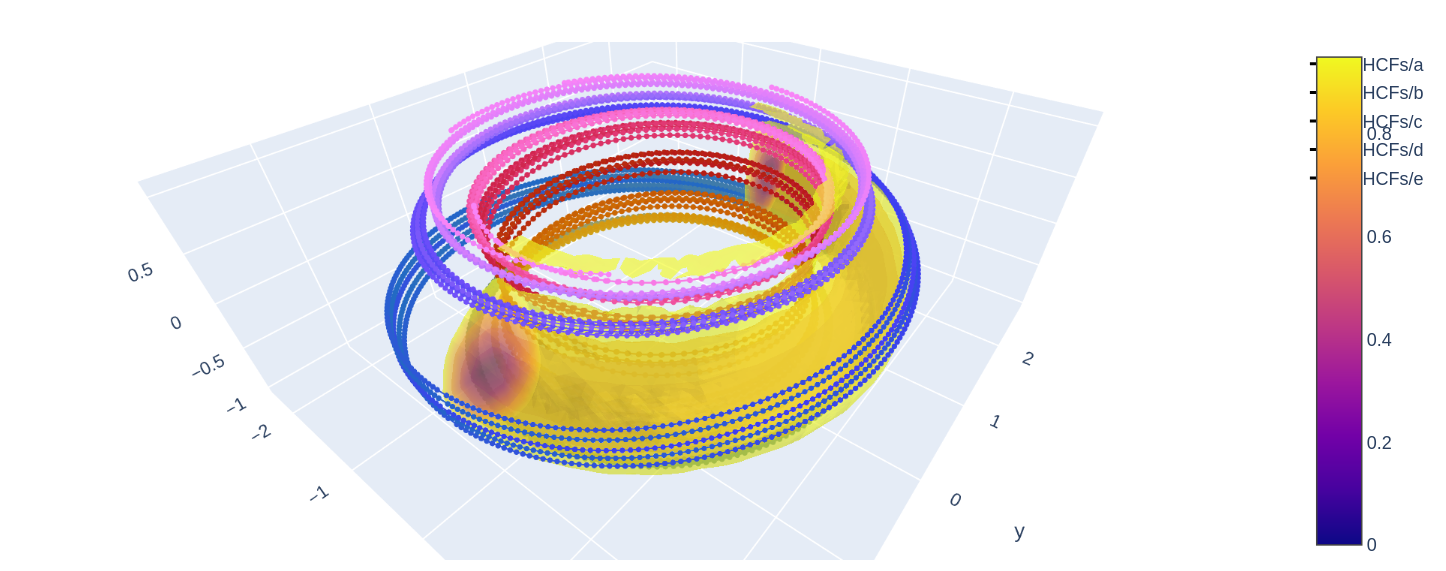
\includegraphics[width=0.47\columnwidth,keepaspectratio]{73999_030400ms_improved/hcfs_east.png}
%   }\hfill
%   \subcaptionbox{\east 上 RMP 线圈(低 n 线圈)、高 m 线圈及在闭合磁面外 15 mm 余处开始延伸的螺旋电流丝结构图。}{%
%   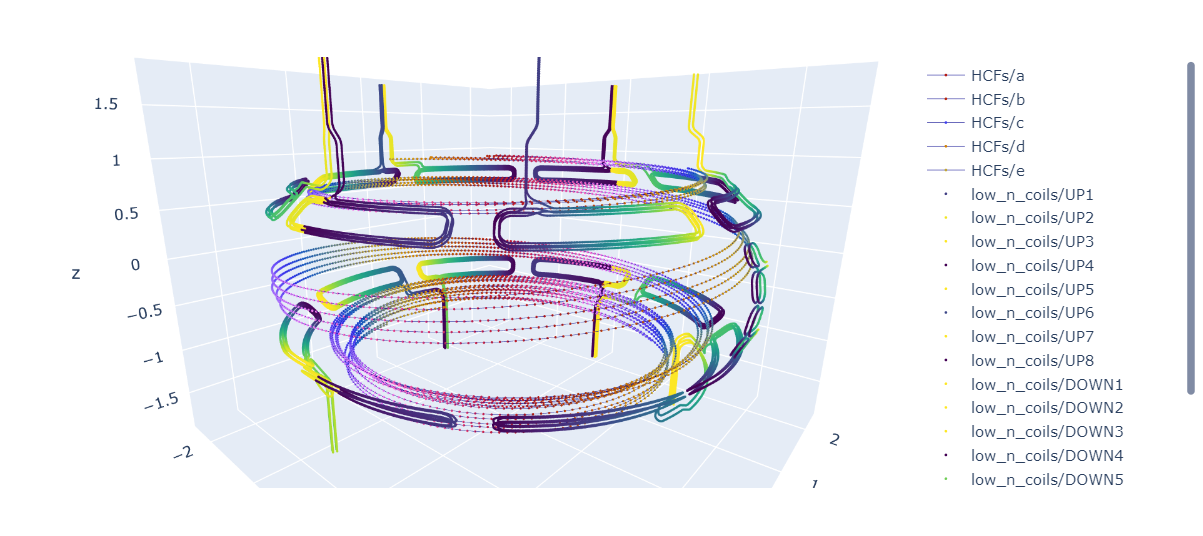
\includegraphics[width=0.47\columnwidth,keepaspectratio]{visual_coilsys.png}
% }
% \end{figure}



  下表罗列除了线圈电流幅值、相位及线圈位置等可调参数的可选空间。
  螺旋电流丝的电流强度和位置实验上不太好控制,将其作为给定量,由其他线圈配合它。

  
\begin{table}[htb]
  \centering
  \caption{扰动场可调参量}
  \label{tab:east_parameter}
  \begin{tabularx}{\linewidth}{lXX}
      \toprule[1.5pt]
      变量 & 备注 & 可选区域 \\
      \midrule[1pt]
      $I_{amp~\text{UP}}$ & RMP 线圈上沿电流幅值 & $[-20 \text{kAt}, 20 \text{kAt}]$\\ 
      $I_{amp~\text{DOWN}}$ & RMP 线圈下沿电流幅值 & $[-20 \text{kAt}, 20 \text{kAt}]$\\ 
      $I_{amp~\text{high m, UP}}$ & 高 $m$ 线圈上沿电流幅值 & $[-10 \text{kAt}, 10 \text{kAt}]$\\
      $I_{amp~\text{high m, DOWN}}$ & 高 $m$ 线圈下沿电流幅值 & $[-10 \text{kAt}, 10 \text{kAt}]$\\
      $\Phi_{UP}$ & RMP 线圈上沿电流相位 & $[-\pi, \pi]$\\
      $\Phi_{DOWN}$ & RMP 线圈下沿电流相位 & $[-\pi, \pi]$\\
      $\phi_{\text{high m}}$ & 高 m 线圈环向分布角 & $[-\pi, \pi]$\\
      \bottomrule[1.5pt]
  \end{tabularx}
\end{table}

实际上能够改变扰动场的即是源的强度和源在环向上的旋转角度,我们通过 Fourier 的性质简化因参数改变带来的计算,主要依据 Fourier 变换的线性性、平移性,大大减少了计算磁谱的成本。

  \begin{itemize}
    \item 线性性:线圈强度的变化,利用傅里叶变换的线性性减少计算量。
    \item 平移性:高 m 线圈的角度是指其自身物理位置在柱坐标系统沿中心轴进行环向上的旋转的角度,在 $(\theta^*, \varphi)$ 上沿着 $\varphi$ 平移 $\Delta\varphi$,利用傅里叶变换的平移性质,相当于$\tilde{b}_{m n}^{1}(s)$乘因子 $e^{-i\left(n \Delta\varphi \right )}$。
    \begin{equation}
      \Delta\varphi \Rightarrow \tilde{b}_{m n}^{1}(s)\times =e^{-i\left(n \Delta\varphi \right )}
    \end{equation}
    $\times =$ 表示原来的 $\tilde{b}_{m n}^{1}(s)$ 需要乘以 $e^{-i\left(n \Delta\varphi \right )}$。

     类似的,如果在极向角度上改变 $\Delta\theta^*$,则可以乘因子 $e^{-i\left(m \Delta\theta^* \right )}$。
     \begin{equation}
      \Delta\theta^* \Rightarrow \tilde{b}_{m n}^{1}(s)\times =e^{-i\left(m \Delta\theta^* \right )}
    \end{equation}
  \end{itemize}  
  


\subsection{优化函数}

    
    这是偏工程方面的优化问题,目标函数有两个条件。一个是尽可能地生成强的边界随机场,这一方面我们用 Chirikov 参数来刻画;另一方面是希望新经典环向粘滞的影响尽可能地小,我们下面给出下面的评估标准。

    \subsubsection{边界平均 Chirikov 参数}

    对 Chirikov 参数在边界取平均,$\langle\sigma\rangle_{s_{1}<s<s_{2}}$ ,通常取 $s_1$ 为 0.9, $s_2$ 为 0.95。该量刻画了等离子体边界的磁岛链的重合程度,本文试图以随机场达到抑制 ELM 的效果,则需要该量尽可能地高。
    

    \subsubsection{品质因子定义}
  品质因子定义 (figure of merit, FoM),
  
  \begin{equation}
    FoM=\left[\frac{\langle\sigma\rangle_{s_{1}<s<s_{2}}^{4}}{\left\langle\sum_{m, n(n \neq 0)}\left[b_{m n}^{r}\right]^{2}\right\rangle_{s_{3}<s<s_{4}}}\right]
  \end{equation}

  其中
\begin{equation}
  b^r = \frac{\vect{B}\cdot\vect{n}}{B_0} = \frac{\vect{B}\cdot \nabla s}{B_0 |\nabla s|}
\end{equation}

我们同样对 $b^r$ 做类似 $\tilde{b}^1$ 的 Fourier 变换

\begin{equation}
  b_{m n}^{r}(s) \equiv \int_{\varphi=0}^{2 \pi} \int_{\theta^{*}=0}^{2 \pi} b^{r}\left(s, \theta^{*}, \varphi\right) e^{-i\left(m \theta^{*}+n \varphi\right)} \frac{d \theta^{*}}{2 \pi} \frac{d \varphi}{2 \pi}
\end{equation}

\begin{equation}
  b^{r}\left(s, \theta^{*}, \varphi\right)=\sum_{m, n=-\infty}^{\infty} b_{m n}^{r}(s) e^{i\left(m \theta^{*}+n \varphi\right)}
\end{equation}

  
其中分母是 $b^r$ 磁谱中分量平方的加和,用它来定性刻画新经典环向粘滞(Neoclassical Toroidal Viscosity, NTV)影响大小。当托卡马克的环向对称性被打破时,会有额外的力矩作用在等离子体上,从而形成共振的环向旋转频率,这被称为新经典环向粘滞效应。

当只考虑基频分量引起的磁岛时,$\sigma\propto \sqrt{I_{coil}}$,Chirikov 参数与扰动场幅值成正比。而$b^r_{mn}\propto I_{coil}$,故而 Chirikov 参数取四次幂作为分子,从而实现了对扰动场的归一化,扰动场的幅度变化不会对该品质因子造成太多的影响。
% 香蕉粒子在等离子体中以香蕉状轨迹往复运动导致的额外的粘性。


% 而关于

% $\tilde{b}_{r e s}^{1}$ The expression that we use for the physical effective radial RMPs is:
% \[
% b_{r e s}^{r} \equiv \frac{\tilde{b}_{r e s}^{1}}{R_{0}\langle\sqrt{g^{11}}\rangle_{\theta^{*}}}
% \]
% where the brackets represent an averaging over $\theta^{*}:\langle\sqrt{g^{11}}\rangle_{\theta^{*}} \equiv \int_{\theta^{*}=0}^{2 \pi} \sqrt{g^{11} \frac{d \theta^{*}}{2 \pi}} .$ 


  % \begin{enumerate}
  %   \item 在边界共振分量较大为好,越在边界产生的共振分量越重要,积分权重与到有理面共振线的距离成反比 $d=dist(point(n,m),q(\Psi_{pol})n)\downarrow, \rho(m,n,q) \uparrow$。
  %   \item 减去或除去芯部有理面的共振分量,减弱 2/1, 3/1 有理面存在的不稳定性反馈。。
  % \end{enumerate}
    
  % \begin{equation}
  %   \int_{\Psi_{pol}>0.87} \sum_{m,n} \rho(m,n,q) |B_{mn}^r| S(\Psi_{pol})d\Psi_{pol} - \sum_{internal~\Psi_{pol}} \sum_{m,n} \rho(m,n,q) |B_{mn}^r|
  % \end{equation}
  
  % 确定了优化函数后通过共轭梯度法找到一个较优解,或者算力允许的话画等位图。
  
    
  % 取磁面坐标$(s=\Psi^{1/2}_{pol},\theta^*,\varphi)$,


    
  
\section{Chirikov 参数优化}

对 Chirikov 的优化相对于考虑 NTV 的磁谱归一化判据而言要更为简单。

\subsection{低 n 线圈}
如果低 n 线圈上侧和下侧基础相位分别为 $\Phi_U, \Phi_L$,那么如果要求它们的极值的连线与磁力线共轭,则要求有 

\begin{equation}
  \frac{\Phi_U - \Phi_L + k\pi /n }{\theta^*_U - \theta^*_L} = q, \quad k\in \mathbb{Z}
\end{equation}

当极值连线指的是极大值和极大值之间的连线时 $k$ 为偶数,当为极大值和极小值之间的连线时 $k$ 为奇数;$n$ 为低 n 线圈工作时的主导模数。

则当 

\begin{equation}
  \Delta\Phi_{UL} = q \Delta\theta^*_{UL} -k \pi /n, \quad k\in\mathbb{Z}
\end{equation}

时与该有理面上磁力线共振,若边界 $0.9<s<0.95$ 处 $q$ 可以视为变化不大,则当 $\Delta\Phi_{UL}$ 满足上式时,共振磁扰动分量较大,从而磁岛半径较大。

低 n 线圈因线圈是离散分布的而不能产生理想的三角函数型扰动,在上述推导中我们相当于假设环向上有无穷的低 n 线圈以削弱这种离散效应。数学上难以描述这种离散效应造成的影响,它会导致当 $\Delta\Phi_{U} $ 和 $\Delta\Phi_{L} $ 变化而 $\Delta\Phi_{UL} $ 不变时,Chirikov 参数也会发生改变。



\begin{figure}[t]
  \centering
  \subcaptionbox{主导环向模数 $n=1$}{%
    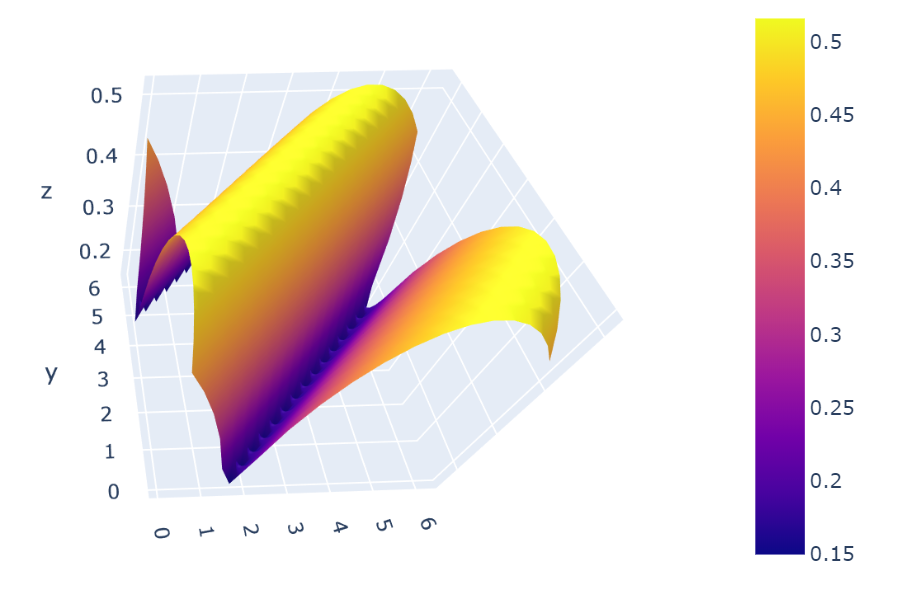
\includegraphics[width=0.47\columnwidth,keepaspectratio]{mean_chirikov/RMP_n_1_10kAt.PNG}
  }%\hfill
  \subcaptionbox{主导环向模数 $n=2$}{%
    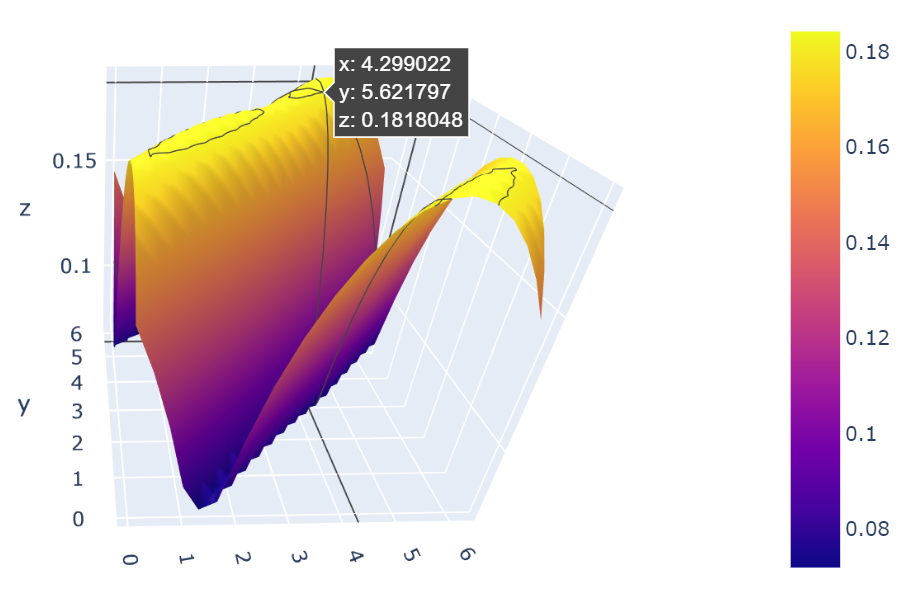
\includegraphics[width=0.47\columnwidth,keepaspectratio]{mean_chirikov/RMP_n_2_10kAt.PNG}
  }%
  
  \subcaptionbox{主导环向模数 $n=3$}{%
  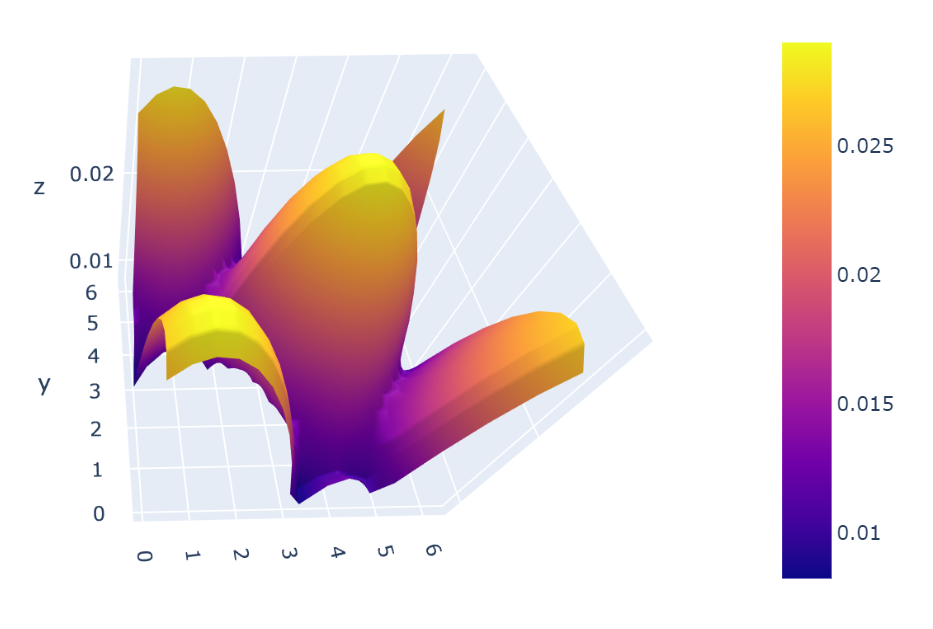
\includegraphics[width=0.47\columnwidth,keepaspectratio]{mean_chirikov/RMP_n_3_10kAt.PNG}
}%
\subcaptionbox{主导环向模数 $n=4$}{%
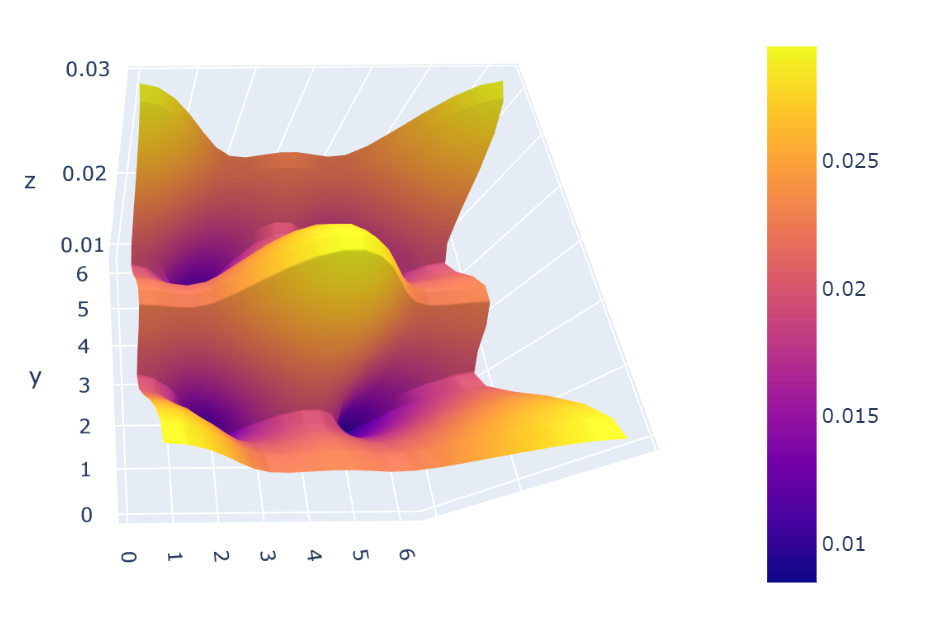
\includegraphics[width=0.47\columnwidth,keepaspectratio]{mean_chirikov/RMP_n_4_10kAt.PNG}
}%
  \caption{低 n 线圈在上下沿基准相位变化($\Phi_U$ 为 x 轴,$\Phi_L$ 为 y 轴)引起的边界 $0.9<s<0.95$ 处平均 Chirikov 参数的变化(z 轴)。}
  \label{fig:lown-multi-n-Phi-scan}
\end{figure}

从图 \ref{fig:lown-multi-n-Phi-scan} 中可见,由于 $n=1$ 的有理面对磁流体的影响最为显著,在同样的电流幅值下,$n=1$ 引起的边界平均 Chirikov 参数是最大的。环向模数越高,越容易因为离散效应出现对称性的破缺。$n=2$ 时该效应不明显,我们用等值线突出其不对称性,$n>2$ 的情况对称性则破缺严重,因为这时八个线圈已经无法满足奈奎斯特采样频率以充分模拟高环向模数 $n>2$ 的三角函数。




\subsection{低 n 线圈与螺旋电流丝}

类似的,在给定了 1kA 螺旋电流丝的背景磁场后,低 n 线圈上下相位与 Chirikov 参数的对应关系也出现了显著的不对称性。即低 n 线圈影响下的 Chirikov 参数不仅与相位差 $\Delta\Phi_{UL} $ 相关,还与相位本身有关,且和上一小节中讨论的离散效应造成的影响略有不同。原本低环向模数时,沿 $\Delta\Phi_{UL} $ 不变的直线 Chrikov 参数亦大致不变,而螺旋电流丝作为非对称扰动场产生的影响是使得该直线有所弯曲,如图 \ref{fig:delta-phi-UL-HCFs-comparision}。

\begin{figure}[t]
  \centering
  \subcaptionbox{无螺旋电流丝}{%
    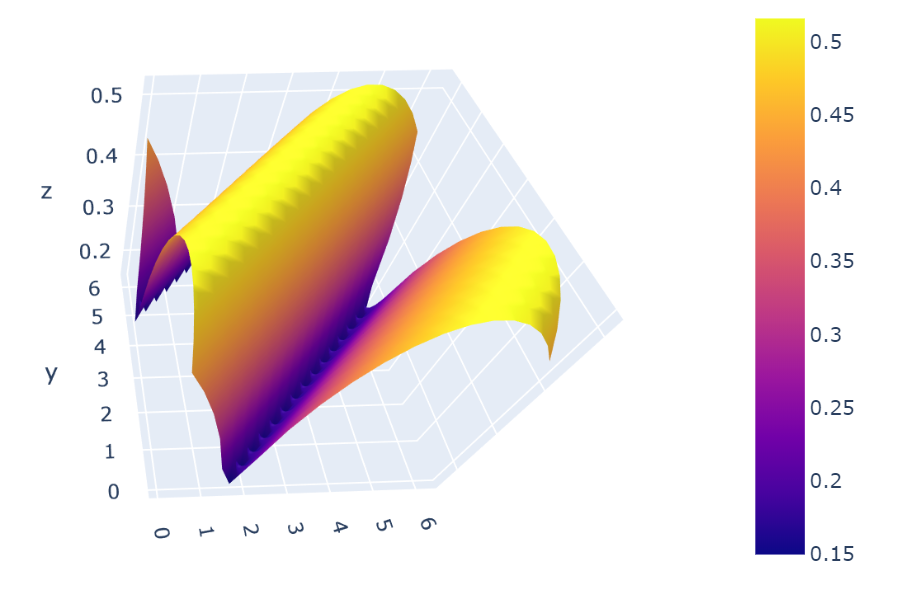
\includegraphics[width=0.47\columnwidth,keepaspectratio]{mean_chirikov/RMP_n_1_10kAt.PNG}
  }%\hfill
  \subcaptionbox{有螺旋电流丝}{%
    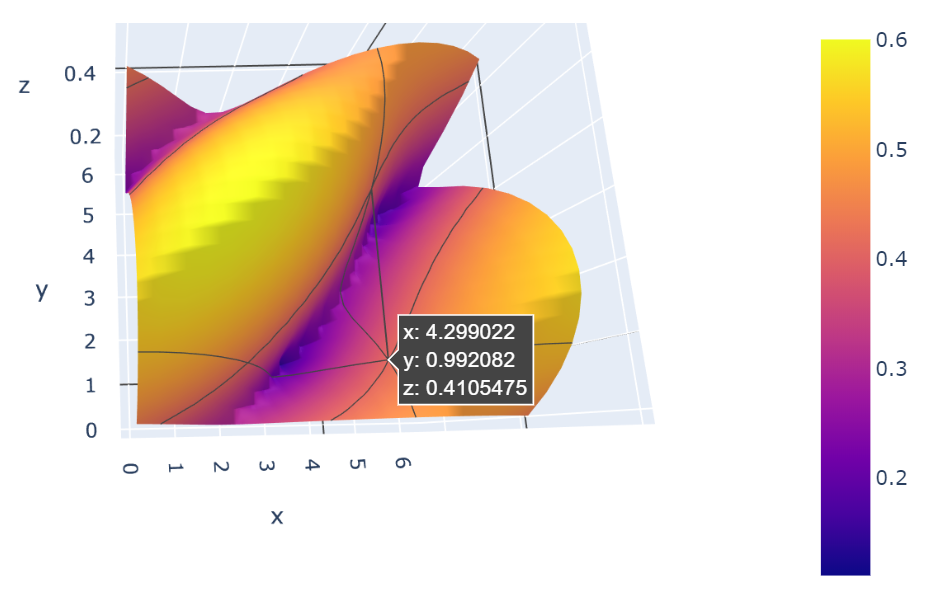
\includegraphics[width=0.47\columnwidth,keepaspectratio]{mean_chirikov/RMP_n_1_10kAt_HCFs_1kA_isoline.PNG}
  }%
  \caption{低 n 线圈(工作模式为主导模数 $n=1$)在无螺旋电流丝和有螺旋电流丝(1kA)两种状况下上下沿基准相位变化($\Phi_U$ 为 x 轴,$\Phi_L$ 为 y 轴)引起的边界 $0.9<s<0.95$ 处平均 Chirikov 参数的变化(z 轴)。}
  \label{fig:delta-phi-UL-HCFs-comparision}
\end{figure}

图中低环向模数 $n=1$ 状态工作时,边界平均 Chirikov 参数有很好的沿直线不变的特性;但是在附加了螺旋电流丝的背景磁扰动后,出现了明显的不对称性,图中标注了等位线表示其已经弯曲。在边界平均 Chirikov 极大值处两者可以协同到达更高的值,而如果不进行设计则可能并无裨益。

当低 n 线圈电流强度不显著时,磁通与螺旋电流丝不匹配,其影响是微弱的,难以起到优化效果。将低 n 线圈的电流幅值从 1kAt 陆续调节到 10 kAt,如图 \ref{fig:chirikov-lown-I-layers},可使得低 n 线圈上下基准相位起到的影响愈加显著。当低 n 线圈电流仅为 1kAt 时,相位基本没有太大的作用,因为背景磁扰动已经有一定的基底。

\begin{figure}[t]
  \centering
    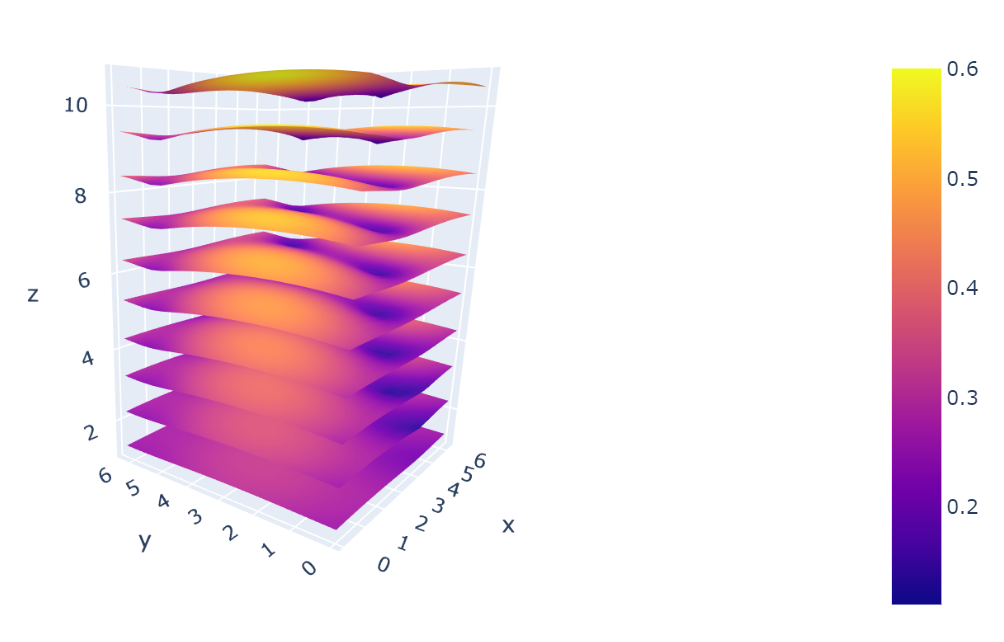
\includegraphics[width=0.7\columnwidth,keepaspectratio]{mean_chirikov/HCFs_1kA_RMP_Phi1_Phi2.PNG}
  \caption{低 n 线圈调节上下沿线圈的相位($\Phi_U$ 为 x 轴,$\Phi_L$ 为 y 轴)引起的 Chirikov 参数的变化,每一层表示不同电流幅值(z 轴,1 kA、2 kA...)的低 n 线圈;z 轴上外加了 Chirikov 参数作扰动使其表现为曲面,以显示不同电流幅值时低 n 线圈的影响强弱。}
  \label{fig:chirikov-lown-I-layers}
\end{figure}

另外,从图 \ref{fig:chirikov-lown-I-layers} 中还可以发现,取极小值处的基准相位是在不断变化的,图中边界处的明暗变化较为明显这表明谱形也在随着电流幅值的大小而改变,表明了螺旋电流丝和低 n 线圈之间协同的可能。

\section{扰动场协同模拟}
此后的协同模拟采用品质因子作为优化参数,先后通过有界优化方法和随机化方法进行求最优解的操作。

\subsection{三者扰动场共同作用}
  
  当首次进行实验时使三种扰动场同时加入到优化中,效果不太理想。磁谱 $\tilde{b}^1_{mn}$ 的脊线和磁面安全因子对应的曲线贴合程度不足,反倒是原本的脊线最高值变得更高了,螺旋电流丝产生的磁场作为基底磁场的影响过大。

  螺旋电流丝基底磁场对应的品质因子已经达到 $3.56 * 10^7$, 优化后可以达到 $4.11 * 10^7$,但倍增的系数不大,意义不是很明显,低 n 线圈没有怎么发挥作用。而不合适地选取低 n 线圈和高 m 线圈的各项参数可能导致该值降到 $10^5$ 的量级。 


  \begin{figure}[t]
    \centering
    % \subcaptionbox{三种线圈共同优化后的结果,在 EAST 73999 Shot 上的 $|\tilde{b}^1_{m,n=-2}|$ 。}{%
      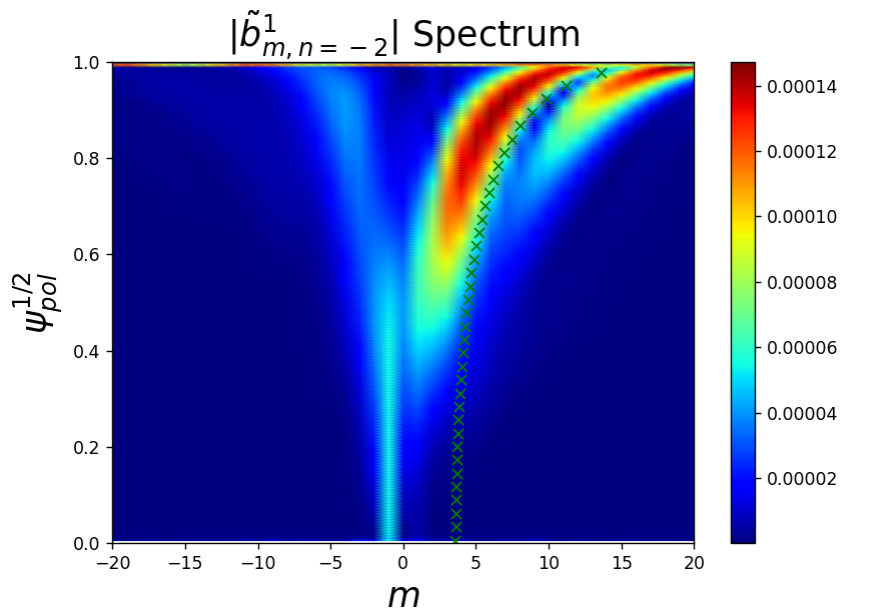
\includegraphics[width=0.7\columnwidth,keepaspectratio]{collab/collab_n=-2_b_sm_nfix_abs.PNG}
    % }
    % \hfill
    % \subcaptionbox{三种线圈共同优化后的结果,在 EAST 73999 Shot 上的 $\tilde{b}^1_{m,n=-2}$ 的相位分布。}{%
    %   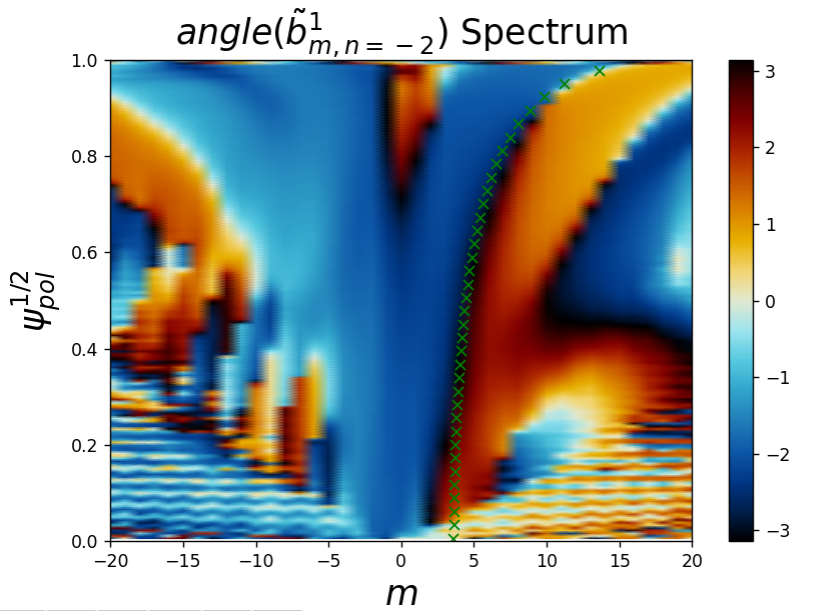
\includegraphics[width=0.47\columnwidth,keepaspectratio]{collab/collab_n=-2_b_sm_nfix_angle.PNG}
    % }%
    \caption{三种线圈共同优化后的结果,在 EAST 73999 Shot 上的 $|\tilde{b}^1_{m,n=-2}|$ 。}
  \end{figure}
  


  
  起初尝试通过 python 科学计算库 scipy.optimize 函数进行优化得到极值, 但结果中低 n 线圈的电流值常常在 1 kAt 以下,但高 m 线圈较大为 -9.01486676 kAt,初步判断可能是陷入了局部极值,但随后用了全局随机遍历亦类似,启发了我们进一步的探索。
  

  
% \begin{figure}[htbp]
%   \centering%
%       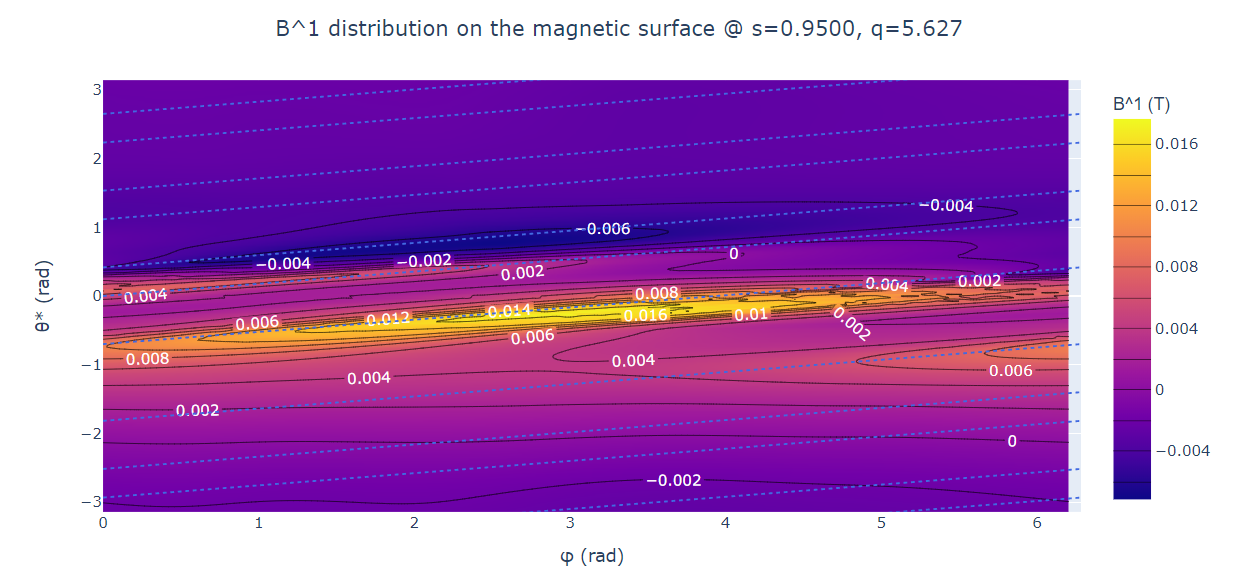
\includegraphics[width=1.0\columnwidth]{hcf/HCFs_uniform.png}
%       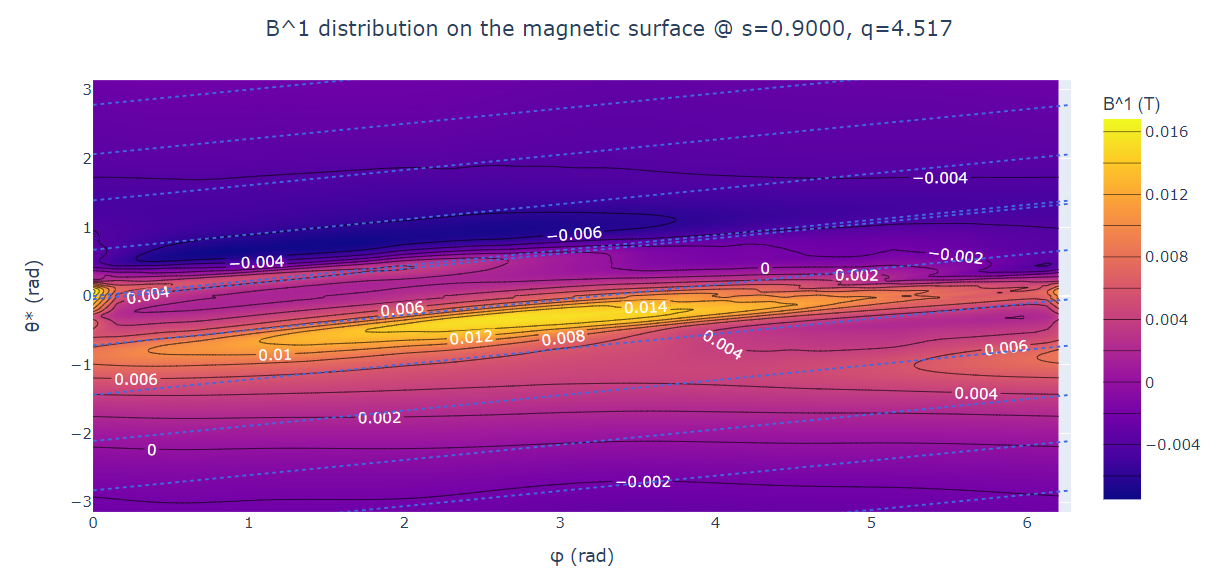
\includegraphics[width=1.0\columnwidth]{collab/collab_n=-2.PNG}
%       \caption{上下图分别为 HCFs 产生的基底磁场和三种扰动场优化后的磁场,各自的 $B^1$ 在磁面上 $s=0.950,0.900$ 的分布。虽然没有控制在一个磁面上,但可见优化后对磁场的影响并不大。}
% \end{figure}
  
% 螺旋电流丝产生的磁场太强,忽略它产生的背景磁场重新测试或者增大 RMP、高 m 线圈电流幅值允许范围。在螺旋电流丝的影响下,磁谱脊线并没有向磁面螺旋度对应的曲线靠拢,反倒是原本的脊线最高值变得更高了。 




\subsection{RMP 线圈与高 $m$ 线圈扰动场共同作用}
上一节随机优化得到的较优值中 RMP 线圈的电流值较小而高 m 线圈较大,这意味着和高 m 线圈相耦合的低 n 线圈强度不能过高,一定程度上告诉我们合适的扰动场需要大小相匹配,比如低 n 线圈(16个)和高 m 线圈(1个)在磁面上的磁通量有数量级的差异,它们应该在磁通量级可比时品质因子有个较好的结果。我们进一步探究这一论断,把螺旋电流丝搁置,先研究低 n (RMP) 线圈和高 m 线圈的协同。

  
  
\begin{figure}[t]
  \centering
  \label{fig:kAt-FoM}
  \subcaptionbox{低 n 线圈上沿 kAt 数 - FoM 散点图}{
      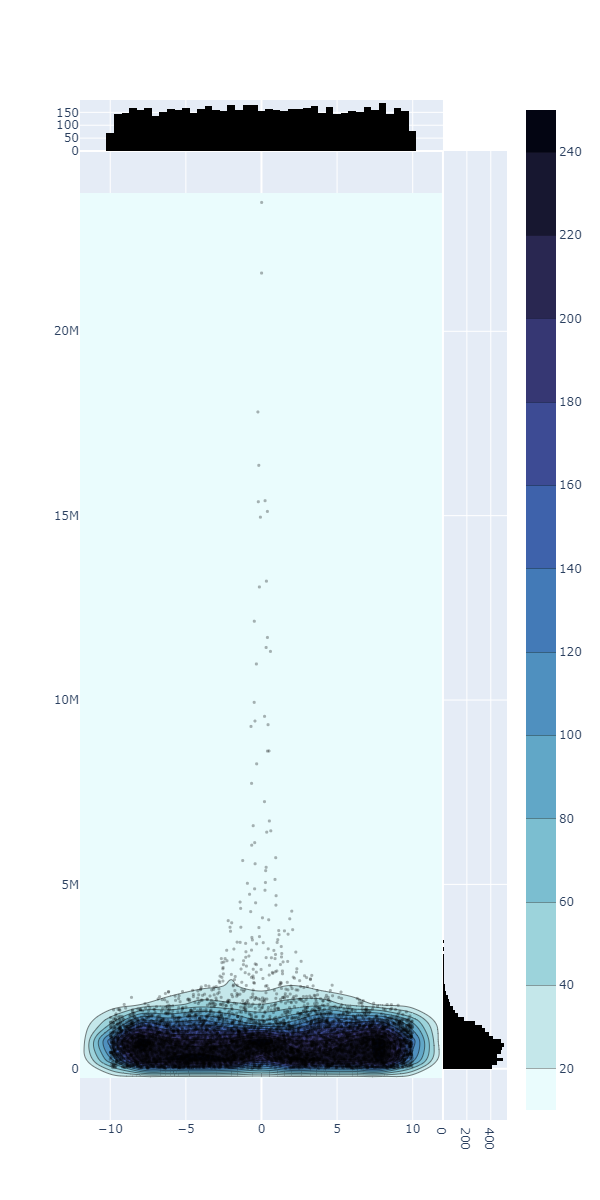
\includegraphics[width=0.32\columnwidth,keepaspectratio]{collab/low_n_UP_FoM.png}
  }%\hfill
  \subcaptionbox{低 n 线圈下沿 kAt 数 - FoM 散点图}{
      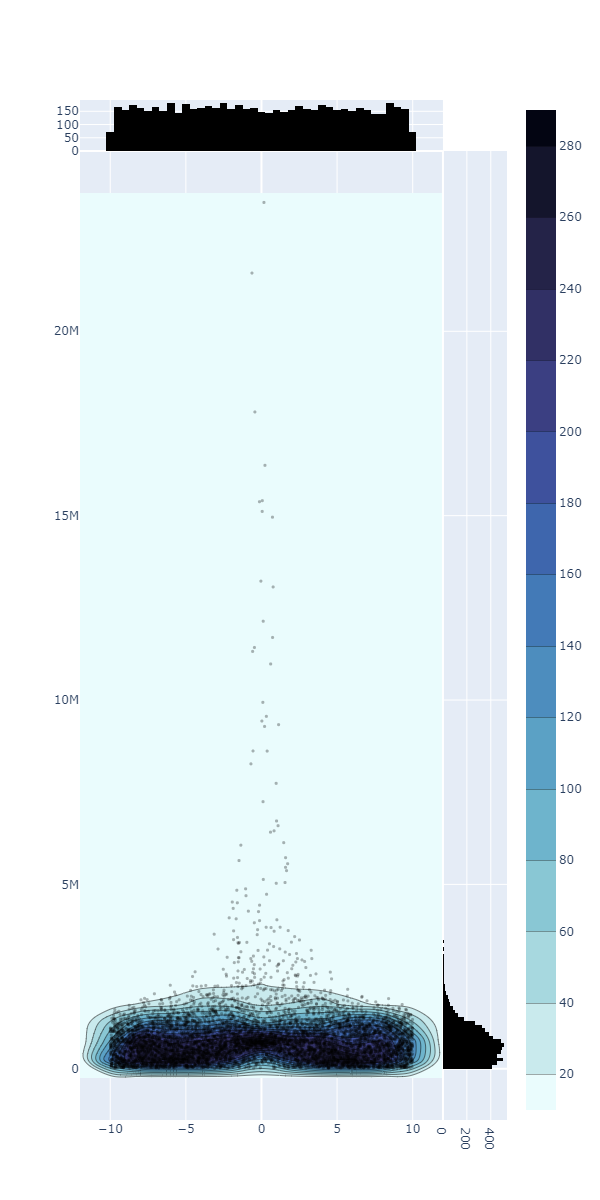
\includegraphics[width=0.32\columnwidth,keepaspectratio]{collab/low_n_DOWN_FoM.png}
  }%\hfill
  \subcaptionbox{高 m 线圈 kAt 数 - FoM 散点图}{
      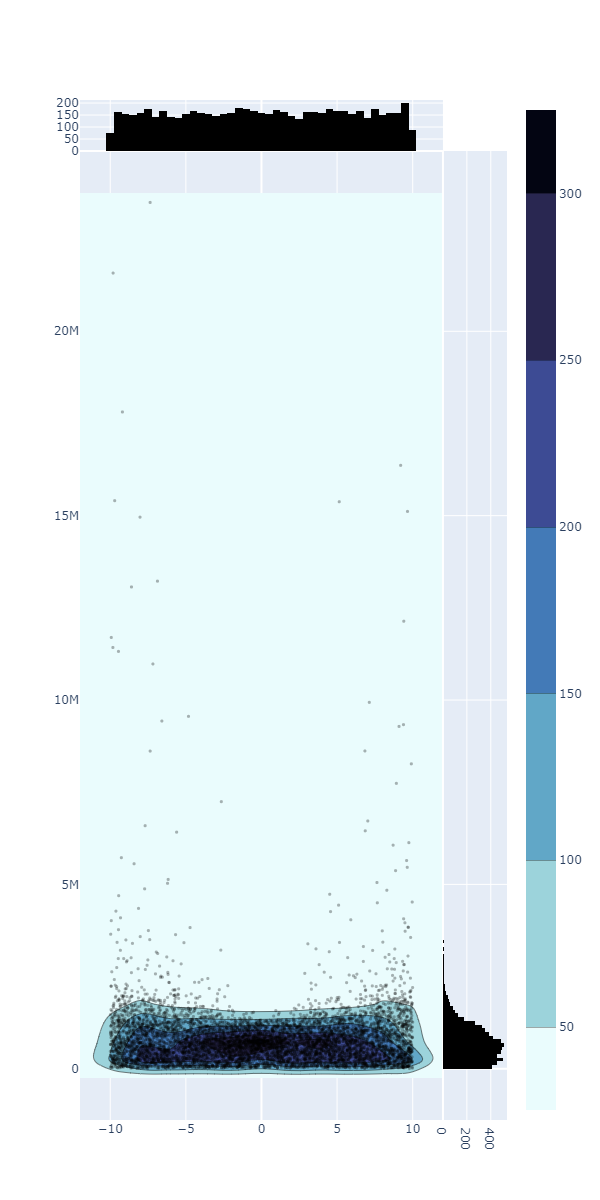
\includegraphics[width=0.32\columnwidth,keepaspectratio]{collab/high_m_FoM.png}
  }
  \caption{低 n 线圈和高 m 线圈随机优化中,各线圈电流幅值对品质因子的影响}
  \end{figure}
  
低 n 线圈和高 m 线圈的协同随机优化发现,线圈电流参数对 FoM 的影响可见图 \ref{fig:kAt-FoM},明显地有着 kAt 数较低 RMP 线圈和较高 kAt 数的高 m 线圈配合有可能产生较高品质因子的趋势。下面转而从各线圈电流幅值、相位和旋转角度作散点图试图发现规律。从数据中发现,以各线圈电流幅值大小作散点图确实有着一定的趋势规律,如图 \ref{fig:lown-highm-scatter},在过滤了较低的品质因子的散点中明确地有一条圆锥形的分布规律,且越接近圆锥的中心品质因子越有可能更高。

  \begin{figure}[htbp]
    \centering%
    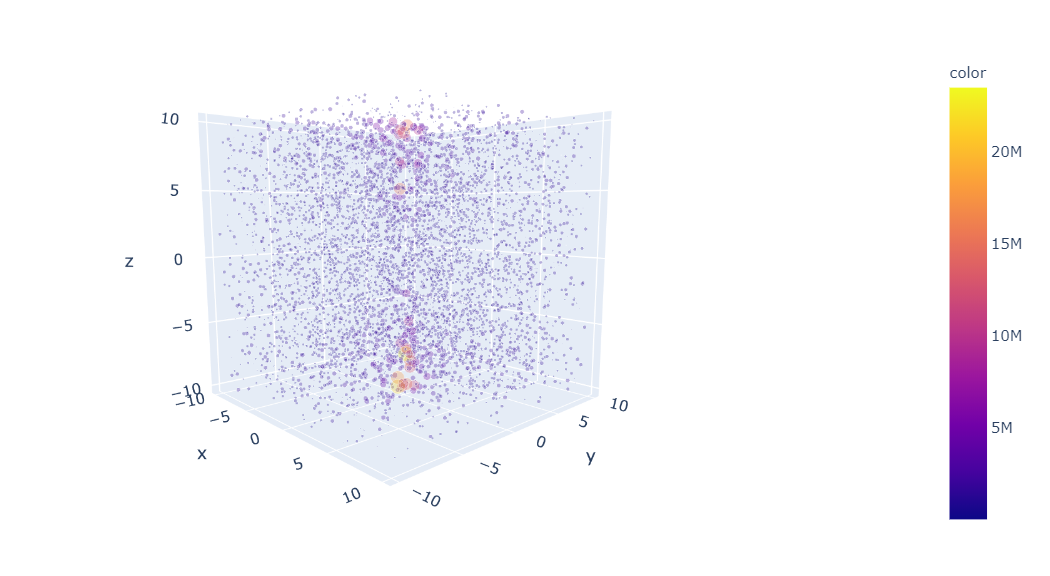
\includegraphics[width=0.55\columnwidth]{collab/Amp_Scatter.png}
    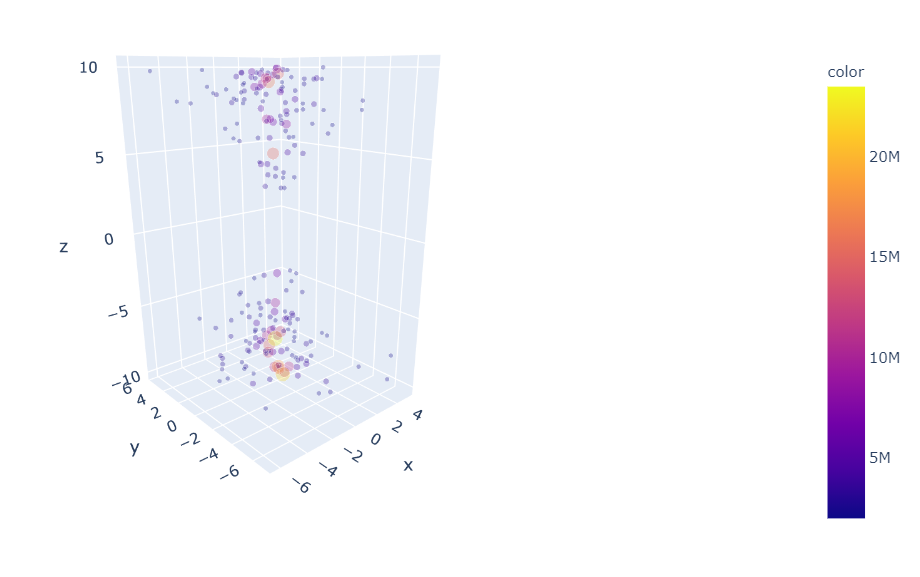
\includegraphics[width=0.42\columnwidth]{collab/Amp_Scatter_FoMthr_2e6.png}
    \caption{左右图均为低 n 线圈和高 m 线圈进行协同优化后得到的品质因子分布,散点的大小和颜色均表示品质因子的大小,坐标轴 XYZ 轴分别为低 n 线圈上下沿的电流幅值和高 m 线圈的电流强度。右图中过滤去除了 FoM 在 2e6 以下的点。}
    \label{fig:lown-highm-scatter}
  \end{figure}

  而以低 n 线圈相位及高 m 线圈旋转角度三者作为坐标轴后作类似上图,未发现明显变化趋势。

  高 m 线圈的电流幅度的增大会导致高品质因子时 RMP 线圈的电流幅值容许范围得以增大,换句话说,即我们需要使得扰动场的“大小”相匹配。扰动场的大小可能很难用一个量来表示,比如螺旋电流丝产生的扰动场可能更看重贡献的极向磁通,而低 n 线圈和高 m 线圈生成径向磁通。关于这方面可能需要更多的研究。

  % \begin{figure}[t]
  %   \centering
  %   % \subcaptionbox{两种线圈共同优化后的结果,在 EAST 73999 Shot 上的 $\tilde{b}^1_{m,n=-2}$ 的绝对值分布。}{%
  %     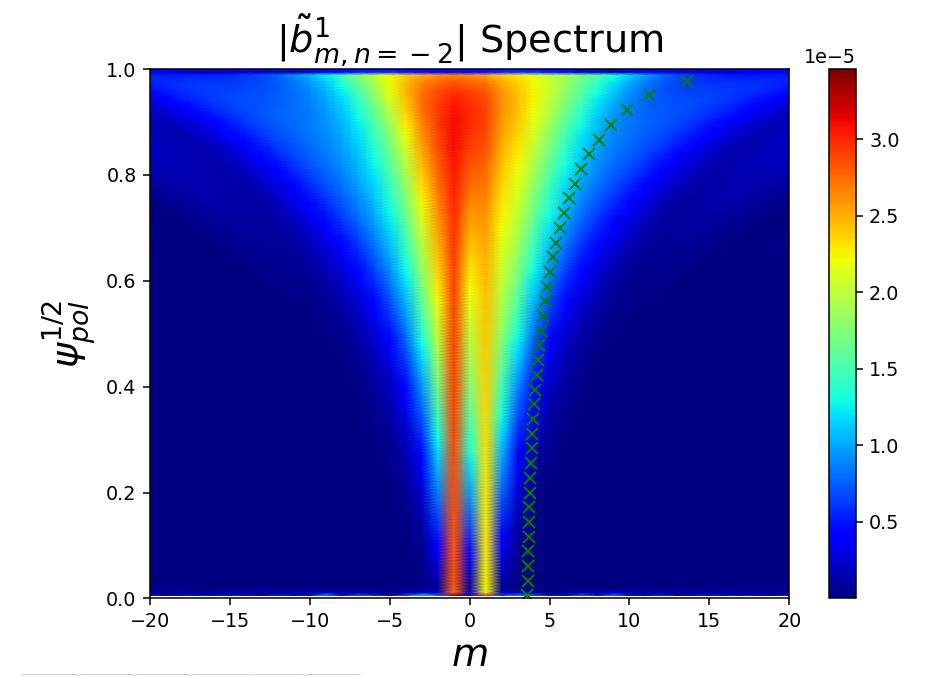
\includegraphics[width=0.7\columnwidth,keepaspectratio]{collab/collab_noHCFs_n=-2_b_sm_nfix_abs.PNG}
  %   % }%\hfill
  %   % \subcaptionbox{两种线圈共同优化后的结果,在 EAST 73999 Shot 上的 $\tilde{b}^1_{m,n=-2}$ 的相位分布。}{%
  %   %   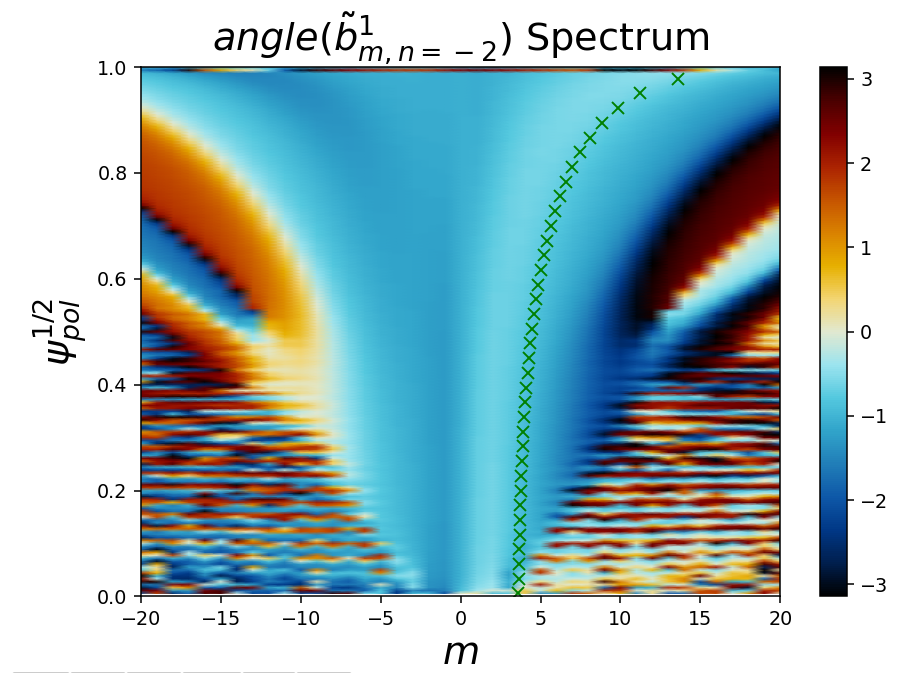
\includegraphics[width=0.47\columnwidth,keepaspectratio]{collab/collab_noHCFs_n=-2_b_sm_nfix_angle.PNG}
  %   % }%
  %   \caption{两种线圈共同优化后的结果,在 EAST 73999 Shot 上的 $\tilde{b}^1_{m,n=-2}$ 的绝对值分布。}
  % \end{figure}
  
  
  


  


    
  
% \begin{itemize}
%     \item 对角度 $\varphi$ 这种有界参数,优化问题可以做一个扫描。但一旦引入了各扰动场的相对大小,优化方法可能就必需了。但 ERGOS 只适合串行,考虑将 ERGOS 中计算 Chirikov 径向分布计算等部分单独抽出来。FFT 可以不抽出来,因为线性性和平移性对每个线圈做一次计算就可以了。
% \end{itemize}


    
  

% 以下对三种扰动场仿真模拟细节陈述。

